\documentclass[tikz,border=2pt]{standalone}
\usepackage{amsmath}
\begin{document}
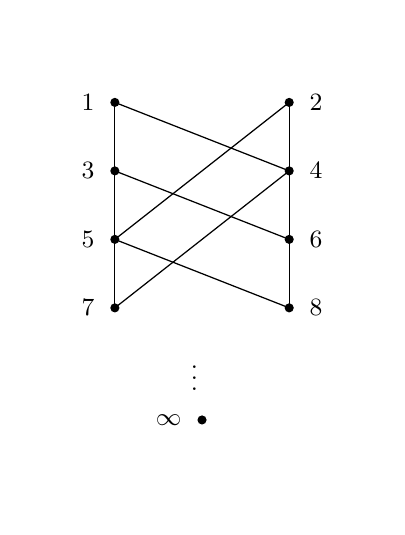
\begin{tikzpicture}[x=.45pt,y=-.45pt,line width=.45pt,line cap=round,font=\fontsize{9}{10}\selectfont]
\path[use as bounding box] (220,15) rectangle (500,400);
\coordinate (nl1) at (290,75);
\coordinate (nl2) at (430,75);
\coordinate (nl3) at (290,130);
\coordinate (nl4) at (430,130);
\coordinate (nl5) at (290,185);
\coordinate (nl6) at (430,185);
\coordinate (nl7) at (290,240);
\coordinate (nl8) at (430,240);
\coordinate (ninfinity) at (360,330);
\draw (nl3) -- (nl1);
\draw (nl4) -- (nl2);
\draw (nl4) -- (nl1);
\draw (nl5) -- (nl3);
\draw (nl5) -- (nl2);
\draw (nl6) -- (nl4);
\draw (nl6) -- (nl3);
\draw (nl7) -- (nl5);
\draw (nl7) -- (nl4);
\draw (nl8) -- (nl6);
\draw (nl8) -- (nl5);
\node at (354,290) {$\vdots$};
\fill (nl1) circle[radius=1.65pt];
\node[anchor=east,inner sep=0pt,fill=white] at (274,75) {$1$};
\fill (nl2) circle[radius=1.65pt];
\node[anchor=west,inner sep=0pt,fill=white] at (446,75) {$2$};
\fill (nl3) circle[radius=1.65pt];
\node[anchor=east,inner sep=0pt,fill=white] at (274,130) {$3$};
\fill (nl4) circle[radius=1.65pt];
\node[anchor=west,inner sep=0pt,fill=white] at (446,130) {$4$};
\fill (nl5) circle[radius=1.65pt];
\node[anchor=east,inner sep=0pt,fill=white] at (274,185) {$5$};
\fill (nl6) circle[radius=1.65pt];
\node[anchor=west,inner sep=0pt,fill=white] at (446,185) {$6$};
\fill (nl7) circle[radius=1.65pt];
\node[anchor=east,inner sep=0pt,fill=white] at (274,240) {$7$};
\fill (nl8) circle[radius=1.65pt];
\node[anchor=west,inner sep=0pt,fill=white] at (446,240) {$8$};
\fill (ninfinity) circle[radius=1.65pt];
\node[anchor=east,inner sep=0pt,fill=white] at (344,330) {$\infty$};
\end{tikzpicture}
\end{document}
